\chapter{Presentación de la solución}

En este capítulo introducimos la solución utilizada para resolver el problema y detallamos su aplicación a la base de datos.

\section{Modelo utilizado}

%Para resolver el problema de conciliación de pronósticos de series de tiempo jerárquicas, utilizamos un modelo lineal respaldado por la función logística. Dado que pretendemos pronosticar el número de viajes en la base de datos de turismo, la función logística se encargará de detectar una tendencia de crecimiento en los viajes.

Para resolver el problema de conciliación de pronósticos de series de tiempo jerárquicas se utilizó el paquete de \textit{fable.tools} el cual a través de optimización busca encontrar la solución óptima al problema de reconciliación. Adicional, ejemplificamos como usar un modelo más robusto para series de tiempo que se adecua con el framework de \textit{fable}. Este método se encuentra implementada en una librería llamada \textit{Prophet}. Dicha libreria fue diseñada por Facebook para realizar pronósticos de series de tiempo a gran escala y es de acceso público mediante Python o R. 

\textit{Prophet} permite realizar pronósticos de series de tiempo basado en un modelo aditivo, donde se puede ajustar tendencias lineales o no lineales con múltiples estacionalidades (anual, semanal, diaria). Adicionalmente, al tratarse de un método aditivo, es posible añadir efectos de vacaciones u otras covariables. Adicionalmente tiene la posibilidad de detectar cambios en tendencia a través de puntos de cambio \cite{taylor2018forecasting}.

La implementación de \textit{Prophet} está basada en la siguiente fórmula, donde g(t) está asociado a la componente de tendencia, s(t) a la componente de estacionalidad y por ultimo, h(t) al efecto de los dias o periodos feriados,  \ref{eq:decomp} (más un factor de error epsilon).

\begin{equation}
    y_t = g(t) + s(t) + h(t) + \epsilon
    \label{eq:decomp}
\end{equation}

\newpage

El modelo fue comparado contra otras técnicas más populares como el suavizamiento exponencial (ETS) y el autorregresivo integrado de promedio móvil (ARIMA) dando buenos pronósticos inclusive ante cambios bruscos de inclinación en las series de tiempo.

\textit{Prophet} implementa 2 modelos basados en tendencia: el modelo de crecimiento saturado y el modelo lineal por partes. En nuestro caso, utilizamos \textit{Prophet} como regresión lineal para pronosticar el número de noches apartadas por visitantes doméstricos a las diferentes regiones y estados de la base de datos de turismo descrita. 

%el primero para determinar el crecimiento en los viajes de la base de datos de turismo, el cual está delimitado por el total de personas (potencialmente mayores de edad).

\section{Implementación}

Utilizando las mejores prácticas descritas en \cite{hyndman2018forecasting} para el desarrollo de pronósticos en series de tiempo, así como los paquetes mencionados previamente, trabajamos el proyecto de la siguiente manera. Como primer paso, agregamos todas las librerias requeridas para el procesamiento de datos. Desde tidyverse, hasta las correspondientes de tidyverts.

\begin{lstlisting}
# Importar librerias requeridas ------
library(tidyverse)
library(tsibble)
library(fable)
library(tsibbledata)
library(feasts)
library(fable.prophet)
library(lubridate)
\end{lstlisting}


\subsection{Generación de TS por agrupación jerárquica}

Como segundo paso utilizamos la función \textit{aggregate\_key()} cuya finalidad es producir una serie de tiempo agregada según niveles de la forma padre/hijo. De esta manera obtenemos un estructura compatible con el enfoque jerárquico para conciliación de series de tiempo. En nuestro problema seleccionamos las variables de agregación \textbf{State} y \textbf{Region} generando grupos sobre la variable \textbf{Purpose}.

\begin{lstlisting}
# Agregar niveles jerarquicos a la base de turismo ------
tourism_aggregated <- 
  tourism %>% 
  aggregate_key((State / Region) * Purpose, Trips = sum(Trips))
\end{lstlisting}

 \begin{figure}[!h]
 \centering
      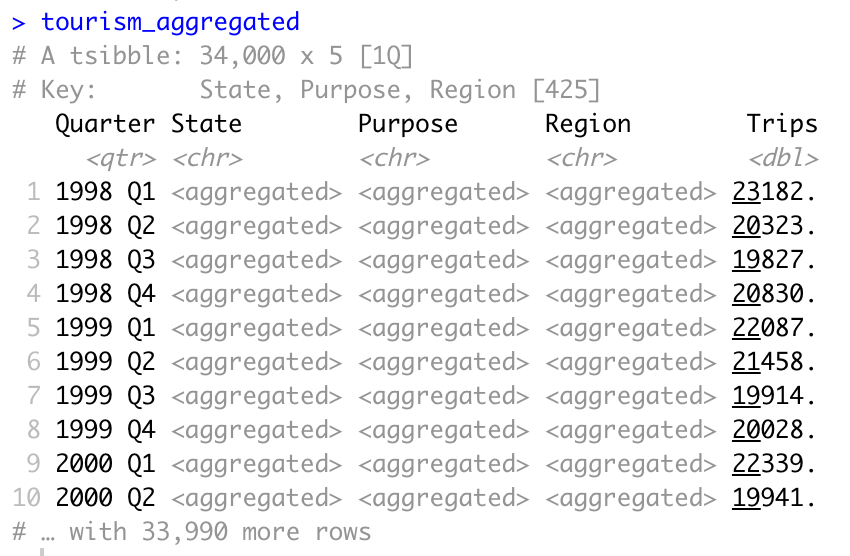
\includegraphics[width=62mm]{imgs/13_aggregated.png}
      \label{fig:snowyplot}
    \end{figure}

\newpage 

Para entender mejor qué realiza esta función, se va a explicar a detalle la salida mostrada. En total se muestran 34,000 registros los cuales podemos detallar en la siguiente tabla:

\begin{table}[!h]
    \centering
    \begin{tabular}{p{2cm}|c|c|c|c|c|c|c}
    Estado  & Propósito & Región & Combin & Registros \\
    \hline
    \hline
    Aggregated & Aggregated &  agreggated  & 1 & 80\\
    Estado & Aggregated &  agreggated  & 8 & 640 \\
    Aggregated & Propósito &  agreggated  & 4 & 320  \\
    Estado & Aggregated & Región  & 76 & 6,080  \\
    Estado & Propósito & Aggregated  & 32 & 2,560  \\
    Estado & Propósito & Región  & 304 & 24,320  \\
    \hline
    Total &  &   & 425 & 34,000  \\
    \hline
    \end{tabular}
    \caption{Número total de combinaciones considerando la jerarquía}
    \label{tbl: res}
\end{table}

Algo importante de mencionar es que el total de combinaciones de no haber considerado las jerarquías, hubiera incrementado en gran número. Esto debido a que el introducir una jerarquía se vuelve una restricción al número de combinaciones. Simplemente, si se consideraran las combinaciones de estado (8), propósito (4) y región (76) hubieran resultado en 2,432 combinaciones, que multiplicadas por los 80 registros, se hubiera tenido más de 190,000 registros.


\subsection{Train - Test split}
Después, separamos los datos en una muestra de entrenamiento y otra de prueba mediante un filtro con la función \textit{yearquarter()} con un punto de corte de  2015 Q1 para poder calcular el accuracy de los modelos. Basados en esto, ajustamos nuestros datos de entrenamiento con modelos clásicos de predicción de series de tiempo como el ETS y ARIMA implementados por las funciones \textit{ETS()} y \textit{ARIMA()} respectivamente. Estos modelos nos servirán de benchmark para evaluar el desempeño del nuestro. Adicionalmente, ajustamos nuestro modelo lineal indicando como variable responsiva el número de noches y como variable predictora el componente estacionario anual. También calculamos un pronóstico combinado al promediar los 3 modelos descritos (\textit{ETS, ARIMA, Prophet}).




\begin{lstlisting}
# Filtrar los datos para poder calcular el accuracy y realizar el fit de los modelos definidos
tourism_fit <- 
  tourism_aggregated %>%
  filter(Quarter < yearquarter("2015 Q1")) %>% 
  model(
    ets_n = ETS(Trips ~ trend("N")), # benchmark
    arima = ARIMA(Trips), # benchmark
    prophet = fable.prophet::prophet(Trips ~ season("year"))
  ) %>% 
  mutate(combn = (ets_n + arima + prophet)/3)
\end{lstlisting}


\textbf{NOTA: es importante considerar que para un adecuado calculo del error no solo hay que considerar una partición de train-test, ya que puede suceder el caso donde el nivel de error depende de la seasonality de la serie de tiempo. En este texto por simplicidad solamente se experimentó con conjuntos de train-test}

\newpage

\subsection{Reconciliación de Forecast Jerárquicos}

Dado que nuestro problema se origina con las series de tiempo jerárquicas, debemos ahora realizar el paso de conciliación para obtener pronósticos coherentes. Esto se logra con la función \textit{reconcile()}, la cual espera el método elegido para conciliar. Nosotros trabajamos con OLS que es un método de combinación óptima el cual calcula la suma ponderada de las predicciones de los nodos del modelo jerárquico. (De acuerdo a Hyndman, el uso de estos métodos depende de la forma de la matriz $\Sigma_h$, ya que es dificil de estimar con $h > 1$. Las soluciones que propone son:)

\begin{itemize}
\item \textbf{OLS: } Ignorar $\Sigma_h$ 
\item \textbf{WLS: } Asumir que $\Sigma_h$ = $k_h \Sigma_1$ es diagonal
\end{itemize}

El alcance de este proyecto considera la alternativa más sencilla, es decir ignorar  $\Sigma_h$, por lo que utilizamos OLS:

\begin{lstlisting}
# Reconciliacion de forecast
tourism_fc_reconciled <- 
  tourism_fit %>% 
  reconcile(coherent = min_trace(combn, method = "ols")) %>%
  forecast(h = "3 years")
\end{lstlisting}

 \begin{figure}[!h]
      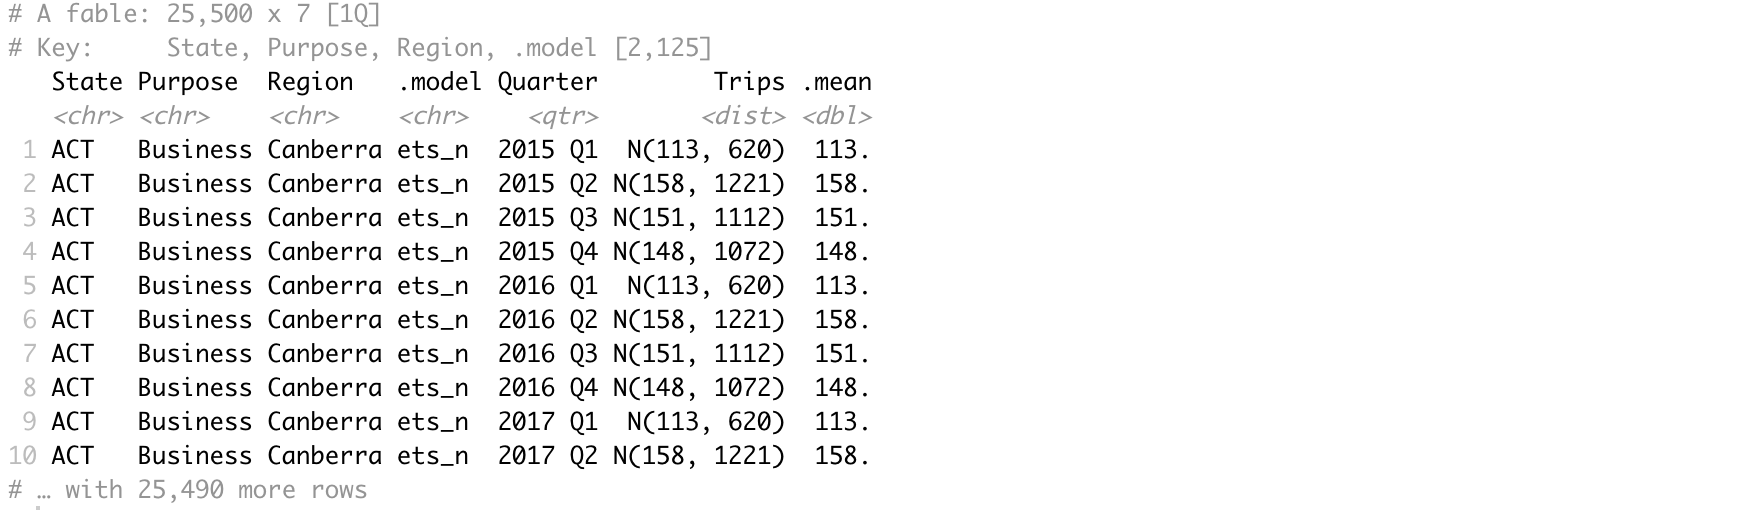
\includegraphics[width=150mm]{imgs/14_reconciled.png}
      \label{fig:snowyplot}
\end{figure}

En la salida anterior, se puede observar que hay 25,500 registros. Como la predicción fue por 3 años, esto implica que cada combinación aparecerá 12 veces (es trimestral). Además, aparecerá 5 veces debido a cada repeticion por modelo (ets, arima, prophet, el promedio de forecast y una extra que es el reconciled). Es decir multiplicamos por 60 cada combinacion. De esta manera podemos presentar la información previa como la tabla \ref{tbl: res1}:

\newpage

\begin{table}[!h]
    \centering
    \begin{tabular}{p{2cm}|c|c|c|c|c|c|c}
    Estado  & Propósito & Región & Combin & Registros \\
    \hline
    \hline
    Aggregated & Aggregated &  agreggated  & 1 & 60 \\
    Estado & Aggregated &  agreggated  & 8 & 480 \\
    Aggregated & Propósito &  agreggated  & 4 & 240 \\
    Estado & Aggregated & Región  & 76 & 4,560  \\
    Estado & Propósito & Aggregated  & 32 & 1,920 \\
    Estado & Propósito & Región  & 304 & 18,240 \\
    \hline
    Total &  &   & 425 & 25,500  \\
    \hline
    \end{tabular}
    \caption{Número total de predicciones considerando la jerarquía}
    \label{tbl: res1}
\end{table}

En la siguiente gráfica, presentamos los pronostcos obtenidos. Por simplicidad, solamente tomamos un Estado y un Propósito de viaje: ''TAS'' (Tasmania), ''Holiday''. En la gráfica se muestra en una linea negra el dato real, en linea azul el dato agregado y en barras el detalle del forecast para cada región. En particular en este estado y propósito se ve una clara estacionalidad en los trimestres. En cada Facet aparece un método distinto, además del coherente:

\begin{figure}[!h]
\centering
      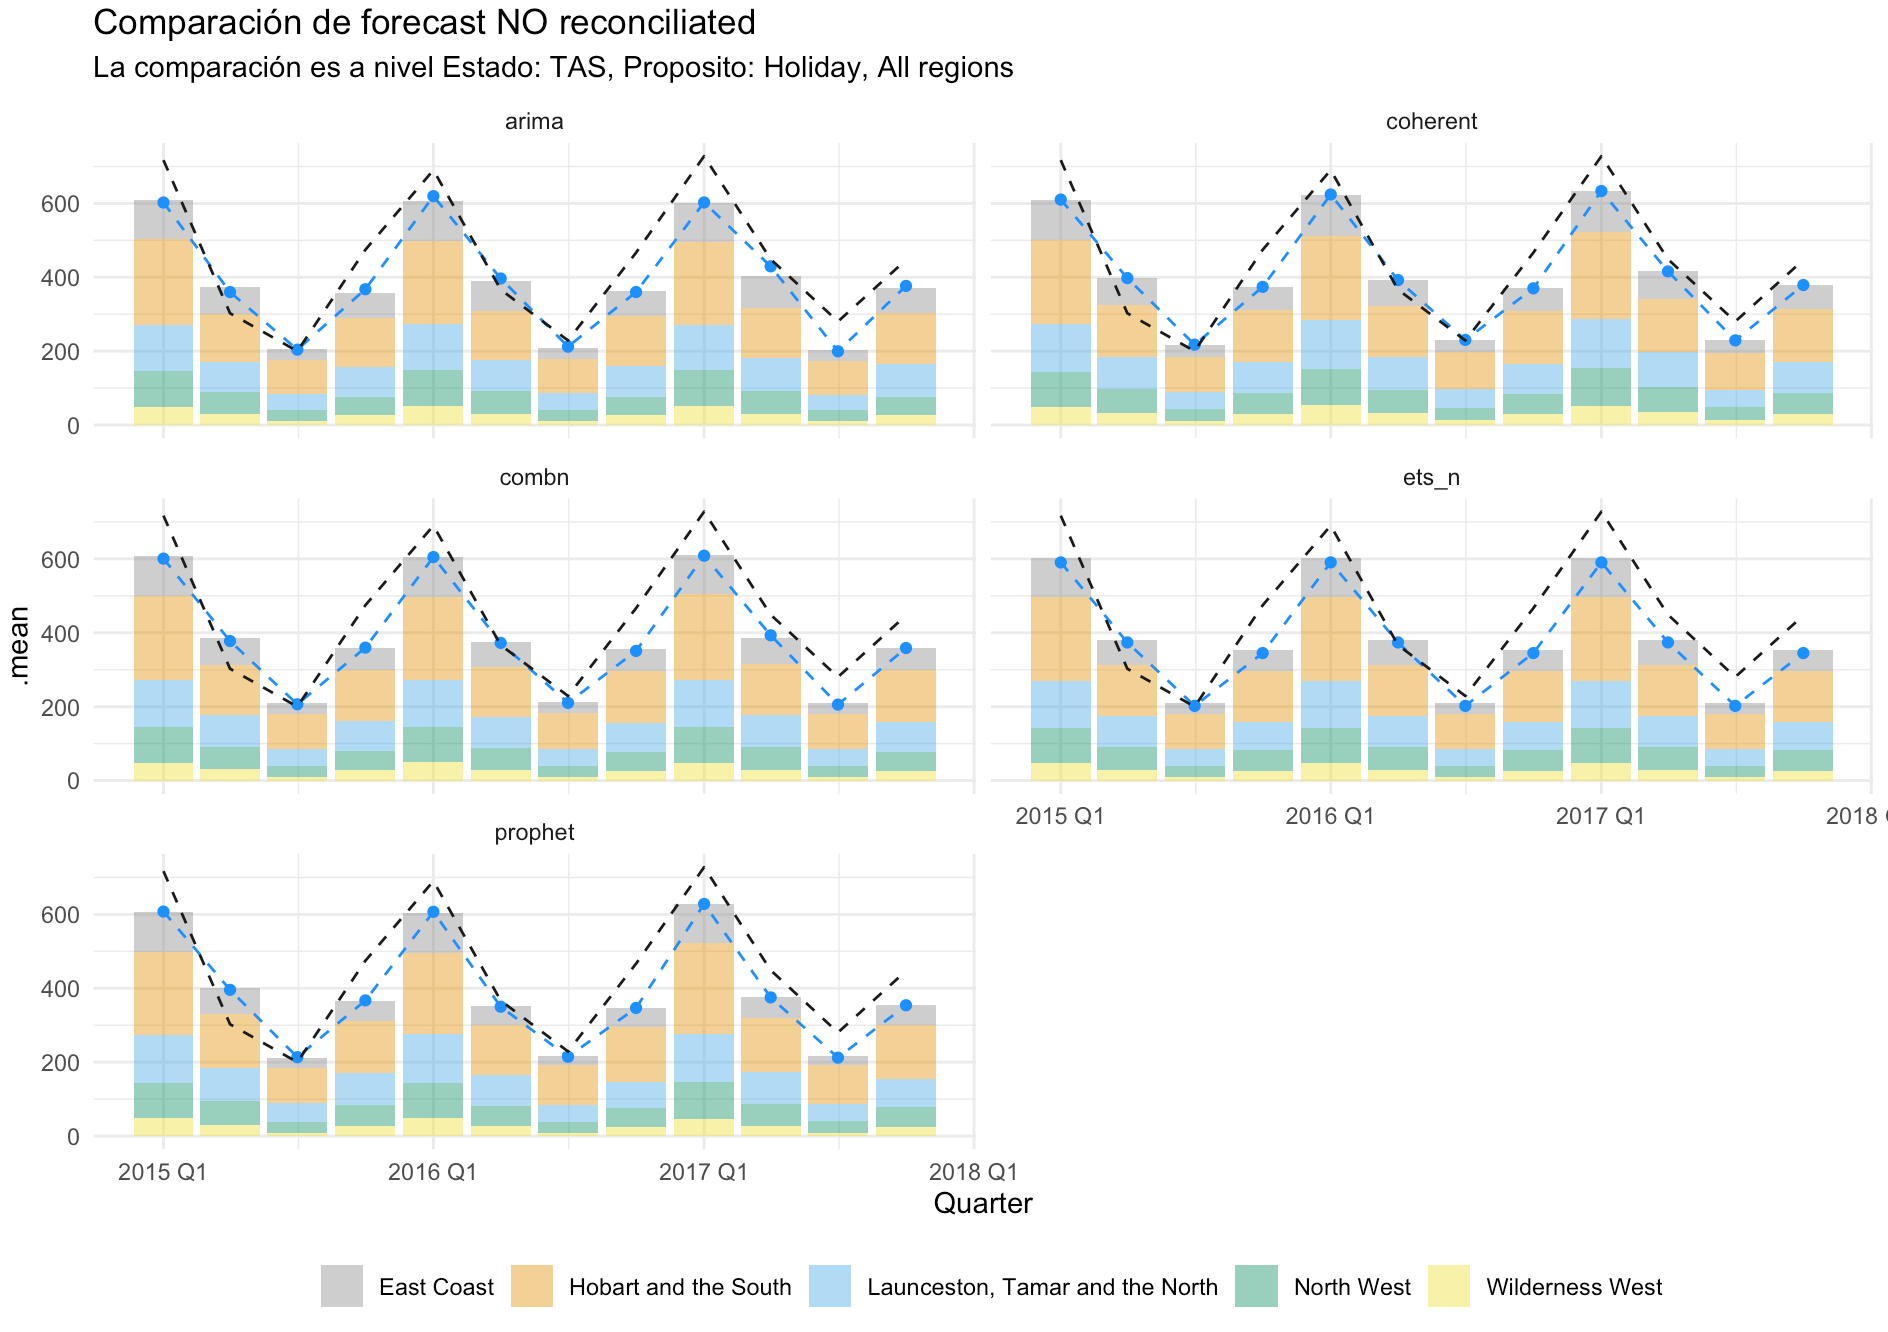
\includegraphics[width=120mm]{imgs/17_no_reconciled_forecast.png}
      \label{fig:snowyplot}
    \end{figure}

\newpage 

La siguiente tabla muestra el detalle para algunas observaciones de la serie anterior. Se puede observar como no existe una coherencia entre el dato agregado y el desagregado.

\begin{figure}[!h]
\centering
      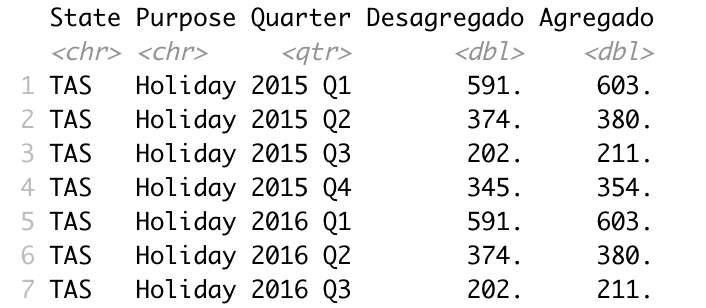
\includegraphics[width=70mm]{imgs/19_no_reconciled_rtable.png}
      \label{fig:snowyplot}
    \end{figure}

Por otra parte, cuando lo comparamos con el modelo coherent (en este caso aplicamos la función reconcile al modelo combinado) se observa que los datos son coherentes entre los niveles de agregación.

\begin{figure}[!h]
\centering
      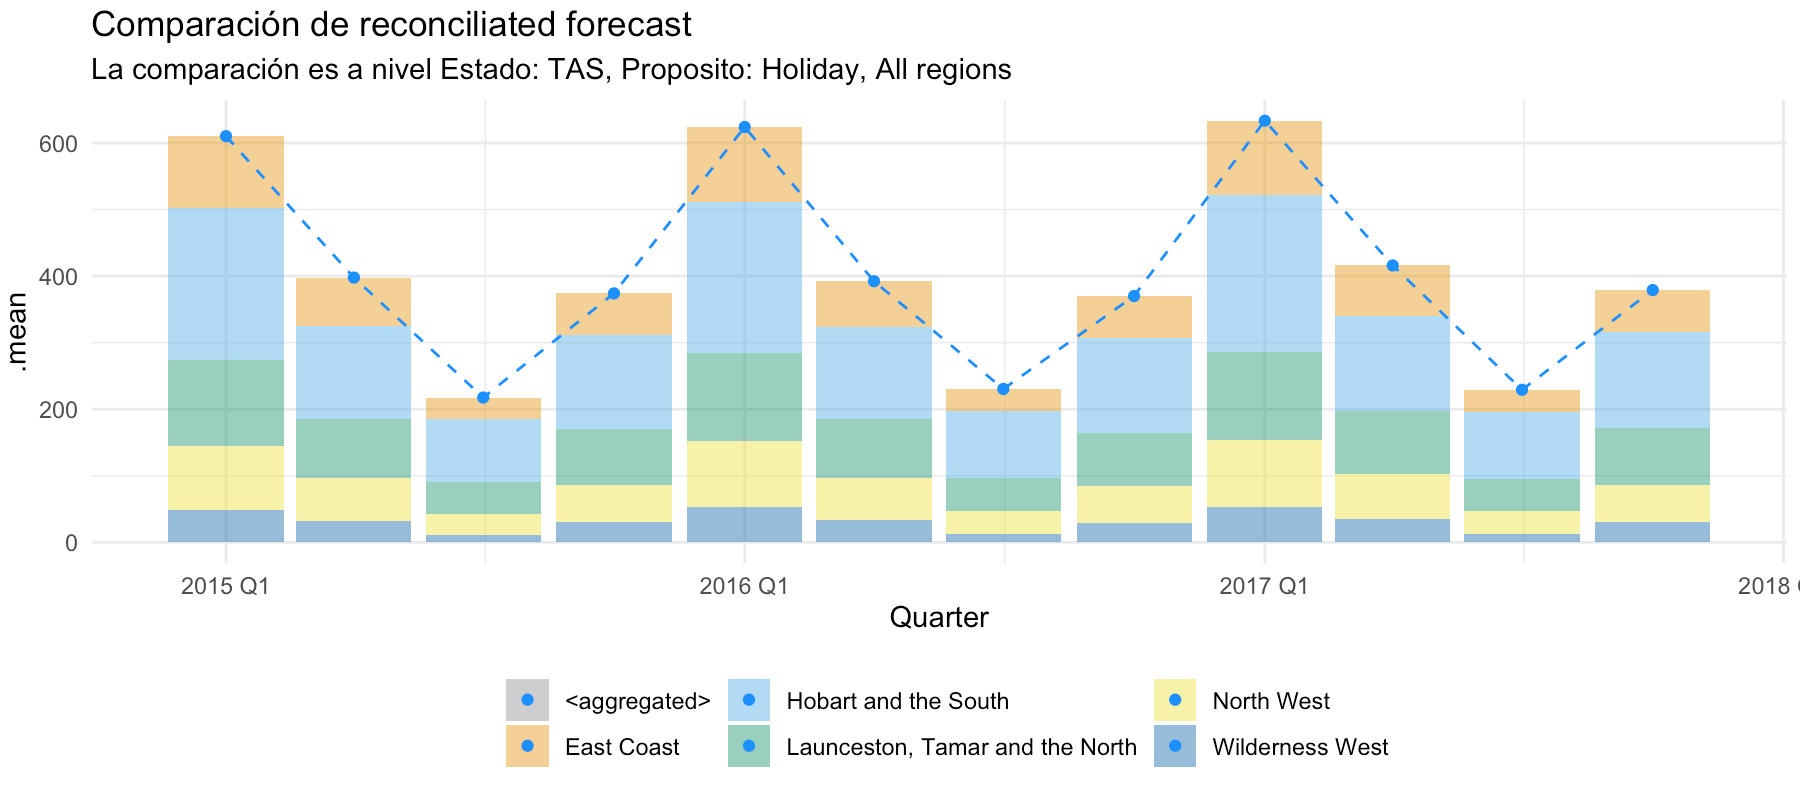
\includegraphics[width=120mm]{imgs/16_reconciled_plot.png}
      \label{fig:snowyplot}
    \end{figure}
    
\begin{figure}[!h]
\centering
      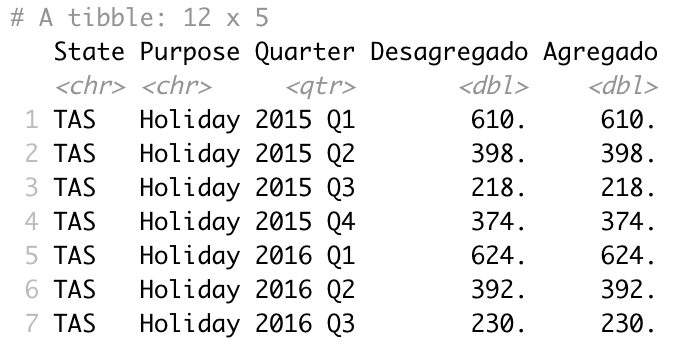
\includegraphics[width=70mm]{imgs/18_reconciled_table.png}
      \label{fig:snowyplot}
    \end{figure}

Algo interesante del método es que se puede realizar la conciliación de cualquier método que se proponga. En la tabla y gráficas mostradas solamente se realizó conciliación del método combinado (combn). 

\newpage 

\subsection{Cálculo de accuracy}

Una vez realizada la conciliación se procede a la fase de cálculo del accuracy, que con el framework de \textit{Tidyverts} también se realiza de manera sencilla. Así, podemos mostrar los modelos de acuerdo a las distintas métricas consideradas:

\begin{lstlisting}
# Calculo del accuracy para cada modelo 
tourism_fc_reconciled %>% 
  accuracy(tourism_aggregated) %>% 
  group_by(.model) %>%
  summarise_at(vars(ME:ACF1), median) %>% 
  arrange(MASE)
\end{lstlisting}

%En este ejemplo se ordena por el MASE (Mean absolute scaled error):

\begin{figure}[!h]
\centering
      
\includegraphics[width=120mm]{imgs/15_MASE_formula.png}
      \label{fig:snowyplot}
    \end{figure}


%¿Prophet es mejor que arima?

%En el documento que describe las características de Prophet \cite{taylor2018forecasting}, los autores mencionan que se realizó un experimento comparando la predicciones de Prophet vs las de un modelo snaive ARIMA del paquete forecasts de R, observando que el modelo benchmark fallaba en capturar los patrones de estacionalidad de largo plazo de la serie, por ejemplo, los modelos naive fueron precisos al capturar patrones semanales de estacionalidad, pero reflejaron fallas al modelar patrones anuales de estacionalidad. Sin embargo, existe documentación informal sobre otros experimentos en los que el modelo ARIMA supera el resultado de Prophet en términos de RMSE.

\begin{table}[!h]
    \centering
    \begin{tabular}{p{2cm}|c|c|c|c|c|c|c}
    Modelo  & RMSE & MAE  & MASE  \\
    \hline
    \hline
    ARIMA &   16.9 & 13.9 & 0.906 \\
    ETS &  15.9 & 13.1 & 0.853 \\
    Prophet &   17.2 & 14.1 &  0.950  \\
    Combinado &  16.4 & 13.6 & 0.896   \\
    Conciliado &  15.0 & 12.4 & 0.872  \\
    \hline
    \end{tabular}
    \caption{Comparación de la evaluación de los modelos utilizados. La conciliación se hizo tomando como base el modelo combinado. Se presentan las métricas de RMSE, MAE, MASE (aunque se pueden utilizar otras)}
    \label{tbl: res2}
\end{table}

\section{Resultados}

En la tabla \ref{tbl: res2} presentamos los resultados obtenidos donde apreciamos que nuestro modelo lineal con \textit{Prophet} se desempeñó bastante similar a los modelos dedicados. Cabe destacar que la combinación de modelos obtuvo los mejores resultados en la mayoría de las métricas. Por ello, la conciliación de las predicciones se realizó tomando como base el modelo combinado.

Dado que estamos trabajando con mismas unidades en todas las series, podemos usar la columna de MAE para comparar. Observamos que el suavizamiento exponencial dio el mejor ajuste, en contraste, nuestro modelo con \textit{Prophet} tiene un punto de diferencia. En el mismo sentido, nuestro modelo se equivoca en promedio en la misma magnitud que el de ARIMA.

Por lo tanto, podemos decir que la implementación con ML del pronóstico de datos de series de tiempo es comparable con los métodos clásicos de estadística para este problema. Asimismo, en cuanto a la conciliación de las predicciones de la jerarquía, podemos ver que el acercamiento combinado mejora el desempeño con respecto a sus versiones individuales.

% (tourism_fc_reconciled %>% filter(Region == "Snowy Mountains", Purpose == "Holiday") )%>% autoplot(tourism_aggregated %>% filter(Region == "Snowy Mountains", Purpose == "Holiday", Quarter < yearquarter("2015 Q1")),level=NULL)
% La imagen Rplot.png tiene el plot de los m[]etodos para Region: Snowy Mountains, State: New SouthWales, Purpose: Holiday

